\section{Extension}
\label{sec:ext}

\subsection{Sch�ma de la soustraction}
\label{sec:ext1}

\begin{figure}[H]
	\centering
		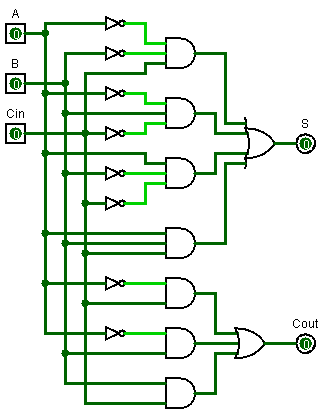
\includegraphics[width=6cm,height=8cm]{./img/soustractor.png}
		\caption{Sch�ma de la soustraction}
	\label{fig:Soustraction}
\end{figure}

\subsection{La soustraction}
\label{sec:ext2}

\paragraph{} La soustraction a �t� impl�ment� � l'ALU, et poss�de son propre code d'instruction pour l'Unit� de contr�le. L'Op�ration est compl�tement op�rationnelle. Cependant par manque de temps et par soucis de conception, nous n'avons pu ajouter le signal sortant de l'ALU indiquant si la sortie �tait n�gative.